\section{Discussion}
\label{sec:discuss}

\begin{figure}[t]
    \vspace{-3mm}
    \begin{center}
    \begin{tabular}{c}
        \hskip2pt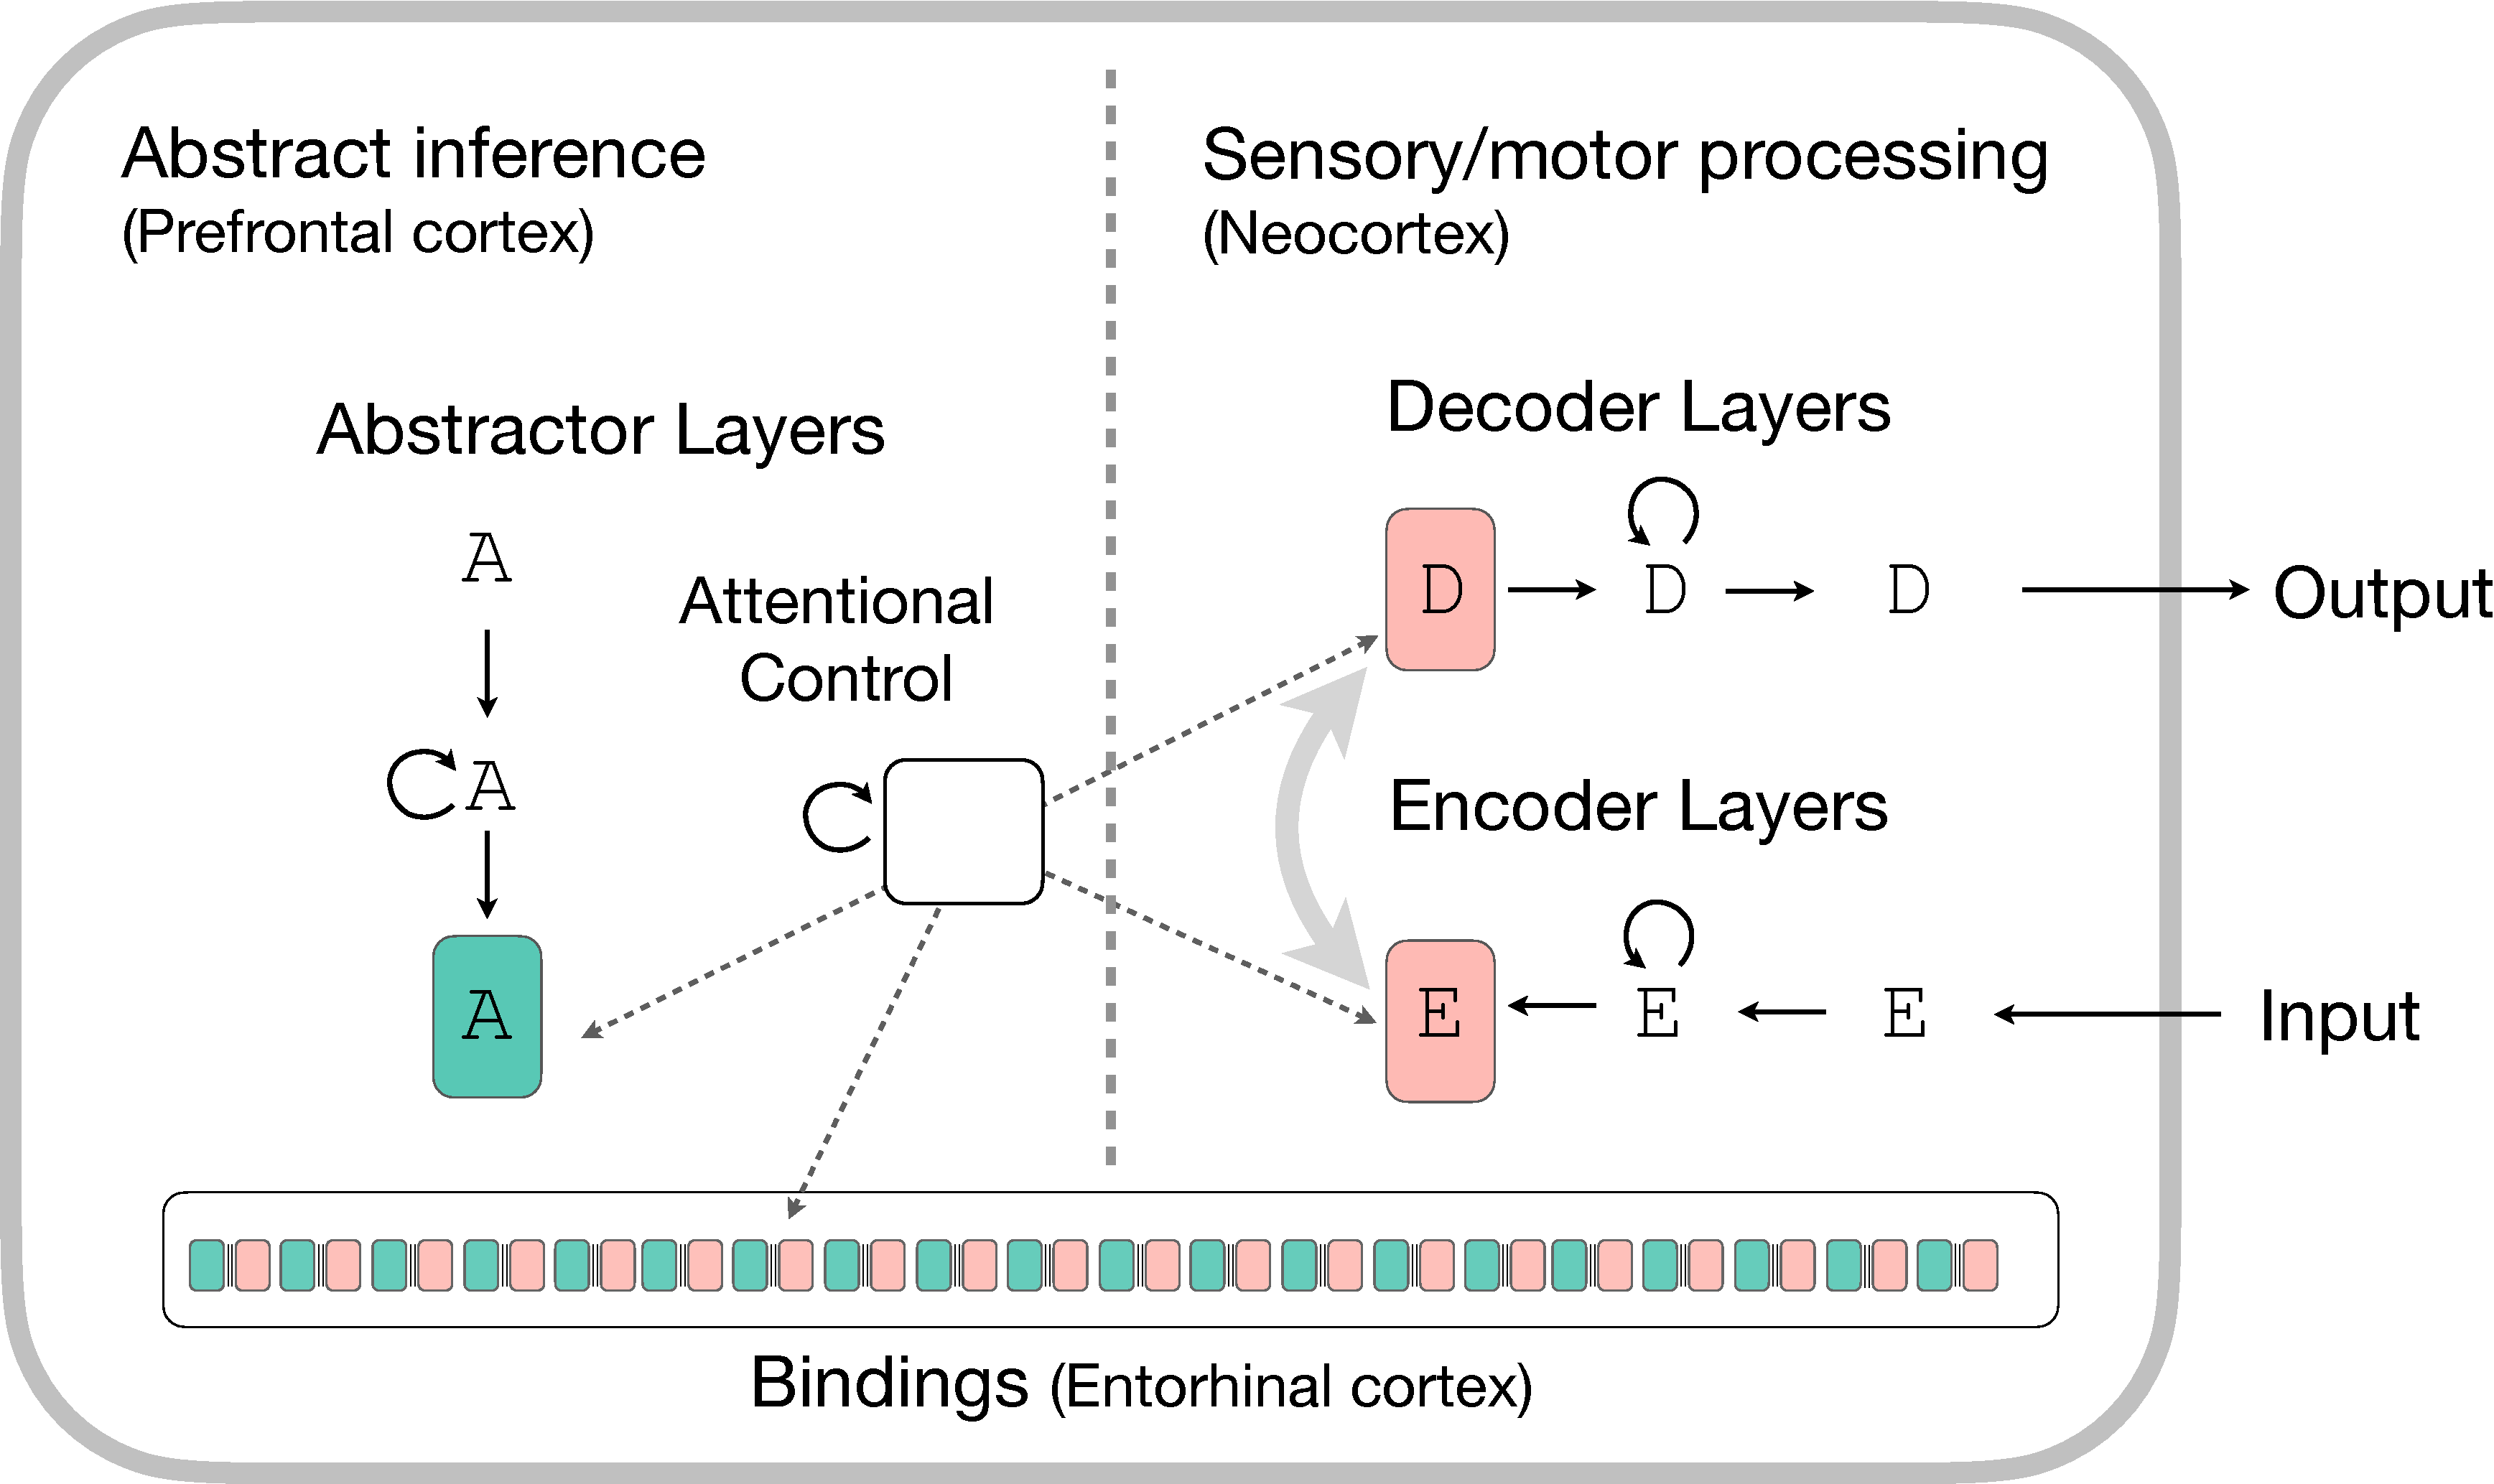
\includegraphics[width=.60\textwidth]{figures/algorithm-diagram2-crop} 
    \end{tabular}
    \caption{In a more general architecture, motivated by principles of information processing 
    in the brain, the relational cross attention mechanisms can be regulated by a controller, and bindings between encoder/decoder and abstractor states are maintained in episodic memory. This allows abstract states---e.g., emergent symbols---to be shared and reused across problems and domains. When Encoder/Decoder states appear together repeatedly through experience and replay, the abstract inference circuit can be preempted by a direct connection (gray arrow), leading to computational efficiency and parallelization (i.e., consolidation and automatization).
    }
    \label{fig:algo2}
    \vskip-12pt
    \end{center}
\end{figure}